\chapter{Methods}
\section{The corpus}
Stimuli for the experiments described here were a subset of the IEEE “Harvard” sentences \citep{HarvardSents} drawn from the PNW/NC corpus, as described in \citet{McCloyEtAl2013}.  Based on that study, three talkers were chosen for the present experiments: PNM02, PNM05, and PNM07.  These talkers were selected because the Pacific Northwest male talkers exhibited the largest spread in inherent intelligibility in the corpus, and those three talkers formed the natural endpoints and midpoint of that group (cf. Figure~\ref{fig:dotchart}).

\begin{figure}
	\begin{centering}
	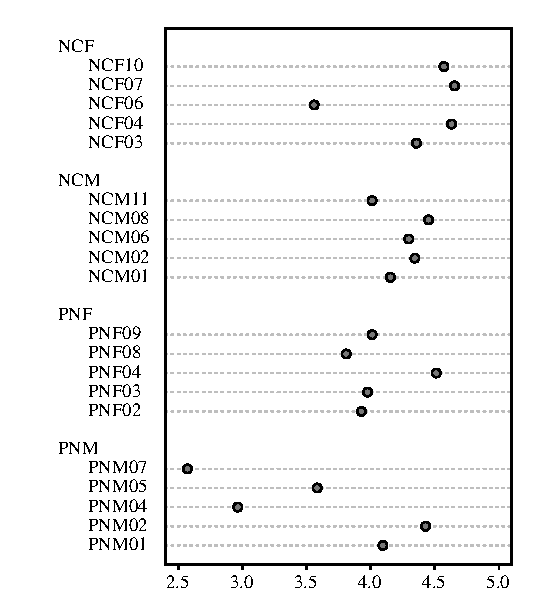
\includegraphics{dotchart.eps}
	\caption{By-talker mean keywords correct (across dialect-matched listeners) in +2 dB SNR condition (adapted from \citet{McCloyEtAl2013}).\label{fig:dotchart}}
	\end{centering}
\end{figure}

\begin{itm}
	\item{description of the sentences}
	\item{characterization of the talkers}
	\item{results of initial intelligibility study \& acoustic modeling}
	\item{method for selection of the 3 talkers used in the remainder of the experiments}
\end{itm}


\section{stimulus design}
\begin{itm}
	\item{duration}
	\begin{itm}
		\item{forced alignment}
		\item{hand-correct forced alignment at syllable level}
		\item{auto extract syllable durations from textgrids}
	\end{itm}
	\item{pitch}
	\begin{itm}
		\item{semiauto pitch settings tool}
		\item{auto pitch object extraction}
		\item{auto manipulation from sound & pitch}
		\item{hand-correct pulses within manipulation}
		\item{auto extract point process from manipulation}
		\item{auto create pitch tier from point process (max interval 0.05 =20Hz)}
		\item{auto replace pitch tier in manipulation object}
		\item{hand-correct pitch tier (spurious low pitch points)}
	\end{itm}
	\item{intensity}
	\begin{itm}
		\item{auto-extract intensity tier}
	\end{itm}
	\item{PSOLA resynthesis}
	\begin{itm}
		\item{dynamic time warping}
		\item{intensity replacement}
		\item{pitch replacement}
	\end{itm}	
\end{itm}


\section{experiment sessions}
Stimuli were presented with a stationary gaussian masker noise, frequency shaped to match the long term spectral average of the corpus of stimuli, at a +2 dB \snr.  To ensure target audibility, the level of the speech was held constant at 68 dB SPL (dB RMS in a 6 cc coupler) and the masker noise was digitally added to the speech to achieve the desired \snr.  The combined signal was presented in a sound-insulated booth over closed-back supra-aural headphones (Sennheiser HD 25–1 II).  Listeners were instructed to repeat each sentence they heard, to give partial answers when they only heard some words, and to guess when they were unsure.  Trials were scored 0–5 on keywords correct during the task.  An audio recording was made of listener responses, and scoring uncertainties were resolved offline by a second researcher.  Talker-sentence-\snr\ assignments were random and unique for each listener, with the following constraints: (a) each listener heard each talker an equal number of times; (b) within each talker, each listener heard each SNR an equal number of times; (c) each listener heard each sentence only once.

\begin{itm}
	\item{subjects}
	\begin{itm}
		\item{number of listeners}
		\item{hearing test}
		\item{dialect controls}
		\item{demographics: age, gender, ethnicity, geography}
		\item{English native; other languages?}
	\end{itm}
	\item{procedure}
	\begin{itm}
		\item{booth, headphones, presentation level}
		\item{task}
		\item{scoring}
	\end{itm}
\end{itm}

\section{data analysis}
\begin{itm}
	\item{mixed effects models (probably logistic)}
\end{itm}
